In this section we begin our investigation of the ratio $R_D$. All the studies we present use use the full information for each LB with the exception of the actual $Z\to (e^+e^-,\mu^+\mu^-)$ counts. The basic strategy, which we implement in small sequential steps, is to use the SM fiducial cross section $\sigma_\text{fid}$ and the measured efficiencies and luminosities, to simulate $Z$ counts in each LB. This part of the analysis is, therefore, completely blinded to Drell-Yan data. We take 
$\sigma_\text{fid} = \sigma_\text{SM}^\text{NNLO} A^\text{MC}_{Z\to \ell^+\ell^-}$, where the NNLO cross section is $\sigma_\text{SM}^\text{NNLO} = 1929\; \text{pb}$ and the Monte Carlo calculated acceptances for electrons and muons are $A^\text{MC}_{Z\to e+e^-} = 0.2996$ and $A^\text{MC}_{Z\to \mu^+\mu^-} = 0.3323224$, respectively.

We label each subsection using the formula used to calculate the corrected $Z$ count. We focus on the muon case only.

\subsection{\texorpdfstring{$N_Z^\text{corr} = \sigma_\text{fid} \cdot {\cal L}_\text{inst}\cdot  \Delta t$}{NZcorr = sigmafid * Linst * Delta t}}
\label{ssec:all_constant}
We begin by a toy study in which we fix the SM fiducial cross section to $\sigma_\text{fid} = 750\; \text{pb}$ and the instantaneous luminosity to ${\cal L}_\text{inst} = 10^{34}\; \text{cm}^{-2} \text{s}^{-1} = 10^{-2}\;  \text{pb}^{-1} \text{s}^{-1}$. The duration $\Delta t$ of each LB is taken from data. The $Z$ count in each LB (identified by its time stamp $t$) is then constructed as\footnote{$N_Z^\text{corr}$ is the $Z$ count corrected for effects of efficiencies. In this toy study we do not include efficiencies but keep the notation for consistency.} $N_Z^\text{corr}(t) = {\cal P} (\sigma_\text{fid} \cdot {\cal L}_\text{inst} \cdot \Delta t)$, where $\Delta t$ is the duration of the LB at time $t$ and ${\cal P}$ stands for Poisson sampling. We then choosing a testing period $T$ (sidereal day, solar day, 1 hour) and histogram the $N_Z^\text{corr}(t)$ counts and the luminosities ${\cal L}= {\cal L}_\text{inst} \cdot \Delta t$ in 100 bins of $\text{mod} (t,T)/T \in [0,1]$. The resulting counts are $N_{Z_i}^\text{corr}$ and ${\cal L}_i$ with $i\in[1,100]$. We then construct the ratio 
%
\begin{align}
R_D = \frac{ N_{Z_i}^\text{corr} / \sum N_{Z_i}^\text{corr} }{ {\cal L}_i / \sum {\cal L}_i} \; .
\label{eq:RD}
\end{align}
%
We calculate this ratio separately for data taken in 2015+2016, 2017 and 2018. The three distributions are then stitched together in the range $[0,3]$ as shown in figure~\ref{fig:toy_RD}. We see that the standard deviation of the 100 bins for this example is $\sigma_{R_D} = 1.5 \times 10^{-3}$.

Using the signal formulas discussed in Eqs.~\ref{eq:duXZ}-\ref{eq:cdXY}, we perform a fit to the 12 SME coefficients. The results are shown in figure~\ref{fig:toy_fits}. The central values are not zero because they have been obtained by a single Poisson sampling.

Finally, we perform a Gaussianity check on the distribution of a given sidereal bin (we choose bin 1) by resampling 1000 times. The histogram of $R_D$ in the first bin and various Gaussianity tests are presented in figure~\ref{fig:toy_Gaussianity}.

\begin{figure}[H]
\centering
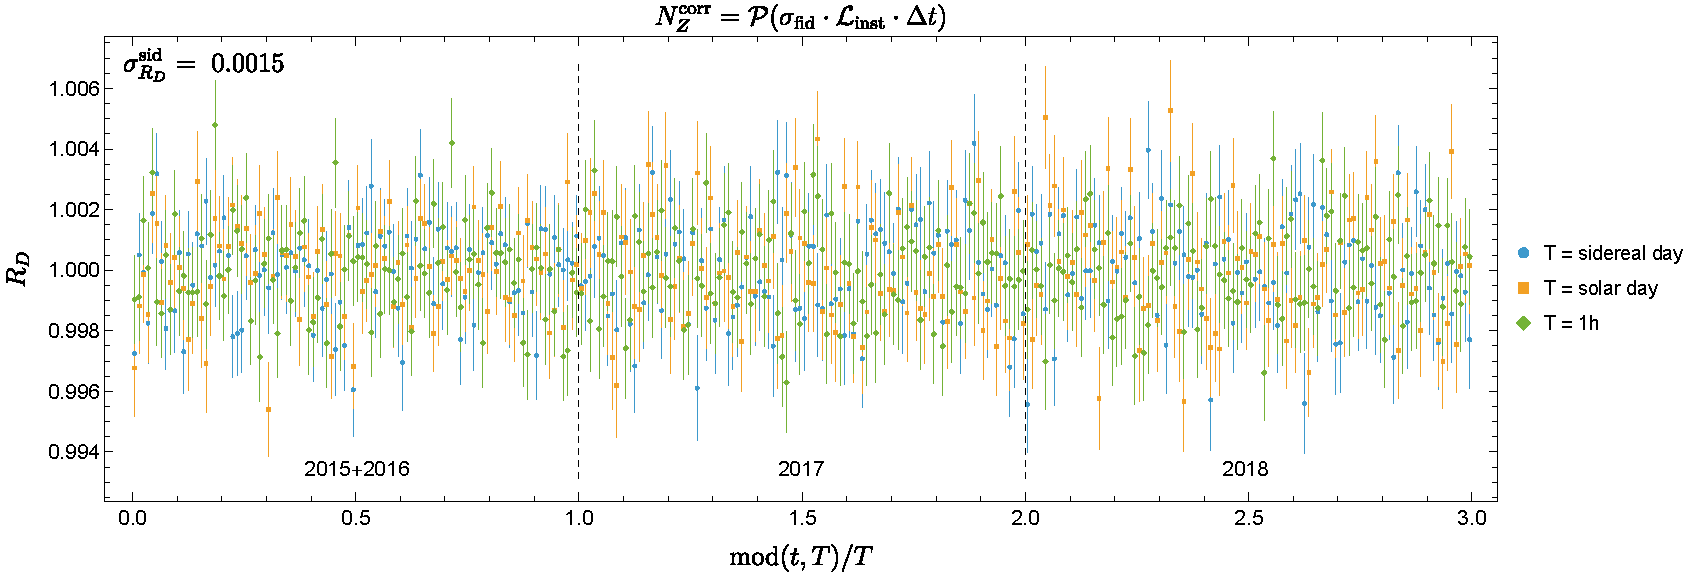
\includegraphics[width=\textwidth]{figs/Mathematica-oldchi2/xs(sigmaFID)_phase(LBlive)}
\caption{$R_D$ distribution for the toy study described in the text. In the upper right corner we show the standard deviation of the sidereal day distribution.}
\label{fig:toy_RD}
\end{figure}

\begin{figure}[H]
\centering
\begin{minipage}[H]{0.49\textwidth}
    \vspace{1.6cm}
    \centering
    \begin{tabular}{|l|c|}
        \hline
        $d_u^{XZ}$ & $(-1.4 \pm 3.0)\times 10^{-6}$ \\
        $d_u^{YZ}$ & $(-1.9 \pm 2.8)\times 10^{-6}$ \\
        $d_u^{XX-YY}$ & $(0.24 \pm 1.6)\times 10^{-6}$ \\
        $d_u^{XY}$ & $(3. \pm 7.7)\times 10^{-7}$ \\
        $c_u^{XZ}$ & $(-1.1 \pm 2.4)\times 10^{-6}$ \\
        $c_u^{YZ}$ & $(-1.5 \pm 2.2)\times 10^{-6}$ \\
        $c_u^{XX-YY}$ & $(0.19 \pm 1.2)\times 10^{-6}$ \\
        $c_u^{XY}$ & $(2. \pm 6.0)\times 10^{-7}$ \\
        $c_d^{XZ}$ & $(-0.48 \pm 1.1)\times 10^{-4}$ \\
        $c_d^{YZ}$ & $(-0.66 \pm 0.98)\times 10^{-4}$ \\
        $c_d^{XX-YY}$ & $(0.8 \pm 5.4)\times 10^{-5}$ \\
        $c_d^{XY}$ & $(1.1 \pm 2.7)\times 10^{-5}$ \\
        \hline
        \end{tabular}
\end{minipage}
\begin{minipage}[H]{0.49\textwidth}
    \vspace{0pt}
    \centering
   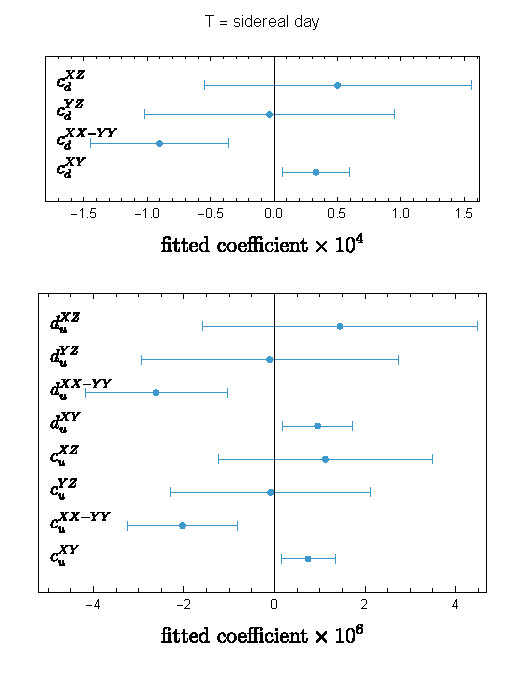
\includegraphics[width=\textwidth]{figs/Mathematica-oldchi2/xs(sigmaFID)_phase(LBlive)_fit}
\end{minipage}
\caption{Fit results for the $N_Z = \sigma_\text{fid} \cdot {\cal L}_\text{inst} \cdot \Delta t$ study.}
\label{fig:toy_fits}
\end{figure}

\begin{figure}[H]
\centering
\begin{minipage}[H]{0.49\textwidth}
    \vspace{0.8cm}
    \centering
   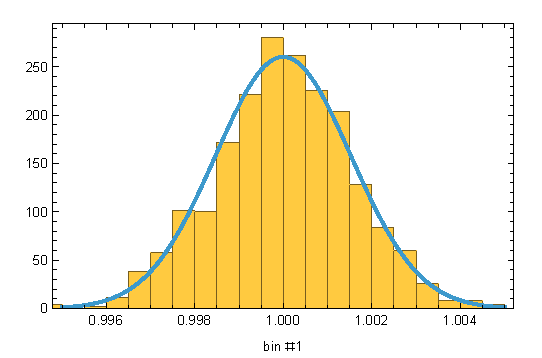
\includegraphics[width=\textwidth]{figs/Mathematica-oldchi2/xs(sigmaFID)_phase(LBlive)_bin1_GaussianityHist}
\end{minipage}
\begin{minipage}[H]{0.49\textwidth}
    \vspace{0cm}
    \centering
    \begin{tabular}{l|ll}
        & \text{Statistic} & \text{P-Value} \\ \hline 
 \text{Anderson-Darling} & 0.418497 & 0.830165 \\
 \text{Baringhaus-Henze} & 0.672449 & 0.459449 \\
 \text{Cram{\' e}r-von Mises} & 0.06435 & 0.786632 \\
 \text{Jarque-Bera ALM} & 0.570246 & 0.748594 \\
 \text{Kolmogorov-Smirnov} & 0.0200947 & 0.806376 \\
 \text{Kuiper} & 0.0353756 & 0.594088 \\
 \text{Mardia Combined} & 0.570246 & 0.748594 \\
 \text{Mardia Kurtosis} & 0.343257 & 0.731405 \\
 \text{Mardia Skewness} & 0.419634 & 0.51712 \\
 \text{Pearson }$\chi ^2$ & 31.424 & 0.445 \\
 \text{Shapiro-Wilk} & 0.99867 & 0.668533 \\
 \text{Watson }$U^2$ & 0.061504 & 0.578408 \\
        \hline
        \hline
        \end{tabular}
\end{minipage}
\caption{Gaussianity checks of the distribution of $R_D$ in the first sidereal bin.}
\label{fig:toy_Gaussianity}
\end{figure}

\subsection{\texorpdfstring{
$N_Z^\text{corr} = \sigma_\text{fid} \cdot \epsilon \cdot F_\text{MC}(\mu)\cdot {\cal L}$ 
with $\delta \epsilon= \delta F^\text{MC}(\mu) = 0$}{NZcorr = sigmafid * epsilon * FMC * L with delta epsilon = delta FMC = 0}}
\label{ssec:no_eFMC_errors}
%
In the next study we include the effects of the efficiency ($\epsilon$) and of the Monte Carlo correction ($F_\text{MC}(\mu)$) to produce a more accurate simulation of the actual $Z$ count. At this stage we take the values of $\epsilon$ and $\mu$ in each LB from data but do not include uncertainties on either $\epsilon$ nor $F^\text{MC}(\mu)$. The dependence of $F^\text{MC}(\mu)$ on $\mu$ is~\cite{ATL-DAPR-PUB-2021-001}:
%
\begin{align}
F^\text{MC}_{Z\to e^+e^-} & = 
\begin{cases}
    0.907628 - 0.000328652\; \mu - 3.0512 \times 10^{-6} \mu^2 & 2015/2016 \\
    0.904096 - 0.000172139\; \mu - 4.35328\times 10^{-6} \mu^2 & 2017 \\
    0.90238 - 8.75767 \times 10^{-5} \mu - 5.79201 \times 10^{-6} \mu^2 & 2018 \\
\end{cases},
\\
F^\text{MC}_{Z\to \mu^+\mu^-} & = 
\begin{cases}
    0.990074 - 5.34716 \times 10^{-6} \mu - 3.23366 \times 10^{-6} \mu^2 & 2015/2016 \\
   0.991619 - 1.21674\times 10^{-4} \mu - 1.58362 \times 10^{-6} \mu^2 & 2017 \\
    0.990808 - 9.99749*10^{-5} \mu - 1.40241 \times 10^{-6} \mu^2 & 2018 \\
\end{cases}.
\end{align}

We construct the simulated $Z\to\mu\mu$ counts for each LB using $N_Z(t) =  {\cal P} ( \sigma_\text{fid} \cdot \epsilon \cdot F^\text{MC}(\mu) \cdot {\cal L})$ and the corresponding corrected count $N_Z^\text{corr} = N_Z(t)/(\epsilon \cdot F^\text{MC}(\mu))$. 

The double ratio $R_D$ is the constructed as in Eq.~(\ref{eq:RD}). The resulting distribution is shown in figure~\ref{fig:RD_noerrors}. The standard deviation of the 100 bins for this example is $\sigma_{R_D} = 1.9 \times 10^{-3}$. Using the signal formulas discussed in Eqs.~\ref{eq:duXZ}-\ref{eq:cdXY}, we perform a fit to the 12 SME coefficients. The results are shown in figure~\ref{fig:RD_noerrors_fits}. The central values are not zero because they have been obtained by a single Poisson sampling.

\begin{figure}[H]
\centering
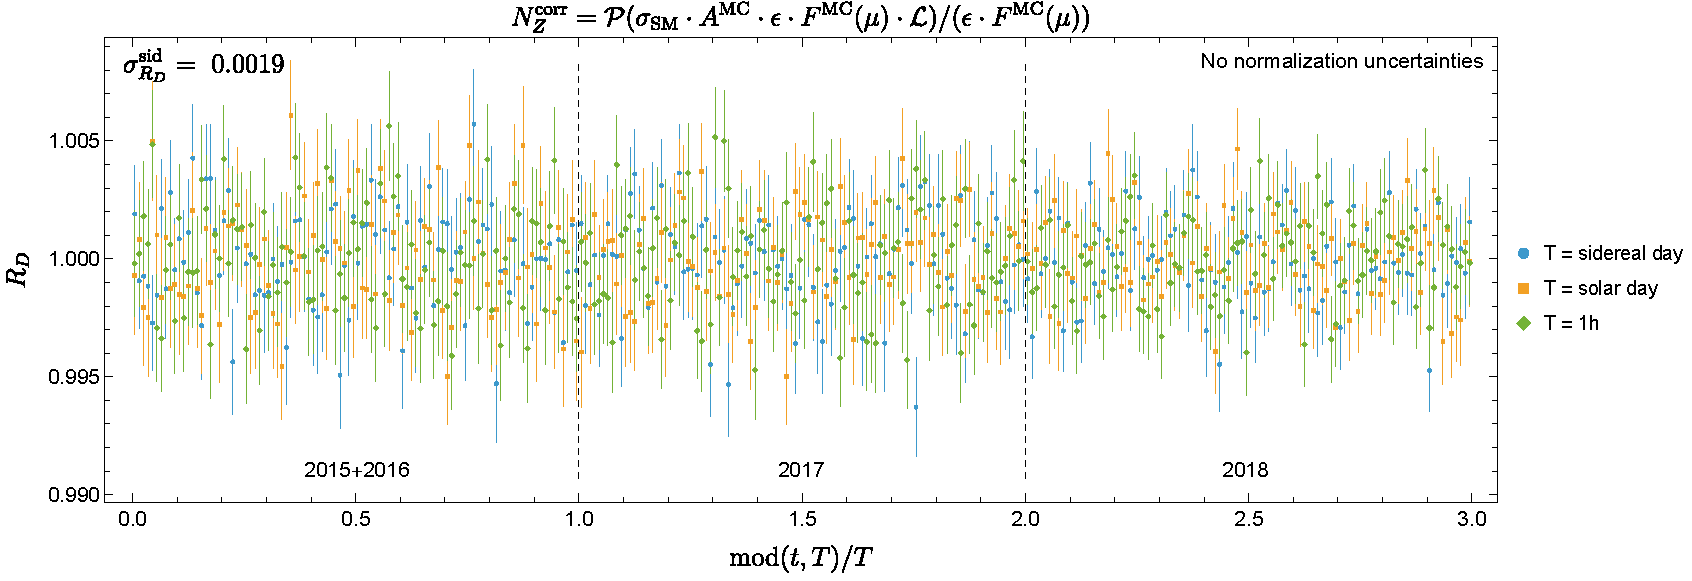
\includegraphics[width=\textwidth]{figs/Mathematica-oldchi2/xs(sigmaFID eps FMC)_noGauss_noNormErr_phase}
\caption{$R_D$ distribution for the toy study described in the text. In the upper right corner we show the standard deviation of the sidereal day distribution.}
\label{fig:RD_noerrors}
\end{figure}

\begin{figure}[H]
\centering
\begin{minipage}[H]{0.49\textwidth}
    \vspace{1.6cm}
    \centering
    \begin{tabular}{|l|c|}
        \hline
        $d_u^{XZ}$ & $(-1.0 \pm 4.0)\times 10^{-6}$ \\
        $d_u^{YZ}$ & $(1.1 \pm 3.8)\times 10^{-6}$ \\
        $d_u^{XX-YY}$ & $(-1.9 \pm 2.0)\times 10^{-6}$ \\
        $d_u^{XY}$ & $(12.7 \pm 9.5)\times 10^{-7}$ \\
        $c_u^{XZ}$ & $(-0.8 \pm 3.1)\times 10^{-6}$ \\
        $c_u^{YZ}$ & $(0.9 \pm 3.0)\times 10^{-6}$ \\
        $c_u^{XX-YY}$ & $(-1.5 \pm 1.5)\times 10^{-6}$ \\
        $c_u^{XY}$ & $(9.8 \pm 7.4)\times 10^{-7}$ \\
        $c_d^{XZ}$ & $(-0.4 \pm 1.4)\times 10^{-4}$ \\
        $c_d^{YZ}$ & $(0.4 \pm 1.3)\times 10^{-4}$ \\
        $c_d^{XX-YY}$ & $(-6.7 \pm 6.8)\times 10^{-5}$ \\
        $c_d^{XY}$ & $(4.4 \pm 3.3)\times 10^{-5}$ \\
        \hline
        \end{tabular}
\end{minipage}
\begin{minipage}[H]{0.49\textwidth}
    \vspace{0pt}
    \centering
   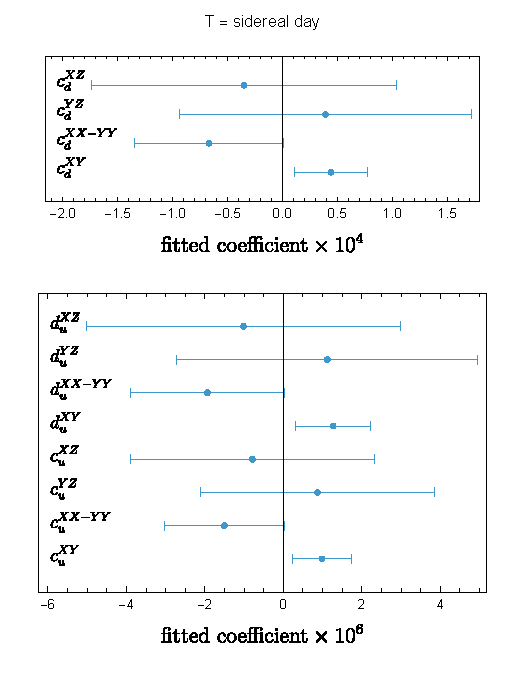
\includegraphics[width=\textwidth]{figs/Mathematica-oldchi2/xs(sigmaFID eps FMC)_noGauss_noNormErr_fit}
\end{minipage}
\caption{Fit results for the $N_Z = \sigma_\text{SM}\cdot A^\text{SM} \cdot \epsilon \cdot F^\text{MC}(\mu) \cdot {\cal L}$. No uncertainties on $\epsilon$ and $F^\text{MC}(\mu)$ are included.}
\label{fig:RD_noerrors_fits}
\end{figure}


\subsection{\texorpdfstring{
$N_Z^\text{corr} = \sigma_\text{fid} \cdot \epsilon \cdot F_\text{MC}(\mu)\cdot {\cal L}$ 
with $\delta \epsilon \neq 0$ and $\delta F^\text{MC}(\mu) = 0$}{NZcorr = sigmafid * epsilon * FMC * L with delta epsilon != 0 and delta FMC = 0}}
\label{ssec:no_FMC_errors}
%
We now repeat the study in Sec.~\ref{ssec:no_eFMC_errors} but including uncertainties on the efficiencies. There are two main changes:
%
\begin{itemize}
    \item In the calculation of the expected number of events (before Poisson sampling) in a given LB we use a value for the efficiency randomly sampled from a Normal distribution corresponding to the measured value $\epsilon \pm \delta \epsilon$ of the efficiency in the given LB:
    \begin{align}
        N_Z (t) = {\cal P} \left( \sigma_\text{fid} \cdot {\cal G} (\epsilon,\delta\epsilon) \cdot F^\text{MC}(\mu) \cdot {\cal L}\right) ,
    \end{align}
    where ${\cal G}(\epsilon,\delta \epsilon)$ stands for Gaussian sampling of a normal distribution with central value $\epsilon$ and standard deviation $\delta \epsilon$.
    \item In the construction of the correct $Z$ count, we propagate the uncertainty from the efficiency:
    \begin{align}
        N_Z^\text{corr} (t) = \frac{N_Z(t)}{(\epsilon \pm \delta \epsilon) \cdot F^\text{MC}(\mu)} .
    \end{align}
\end{itemize}
%
The double ratio $R_D$ is the constructed as in Eq.~(\ref{eq:RD}). The resulting distribution is shown in figure~\ref{fig:RD_noFMCerrors}. The standard deviation of the 100 bins for this example is $\sigma_{R_D} = 2.3 \times 10^{-3}$. Using the signal formulas discussed in Eqs.~\ref{eq:duXZ}-\ref{eq:cdXY}, we perform a fit to the 12 SME coefficients. The results are shown in figure~\ref{fig:RD_noFMCerrors_fits}. The central values are not zero because they have been obtained by a single Poisson sampling.

\begin{figure}[H]
\centering
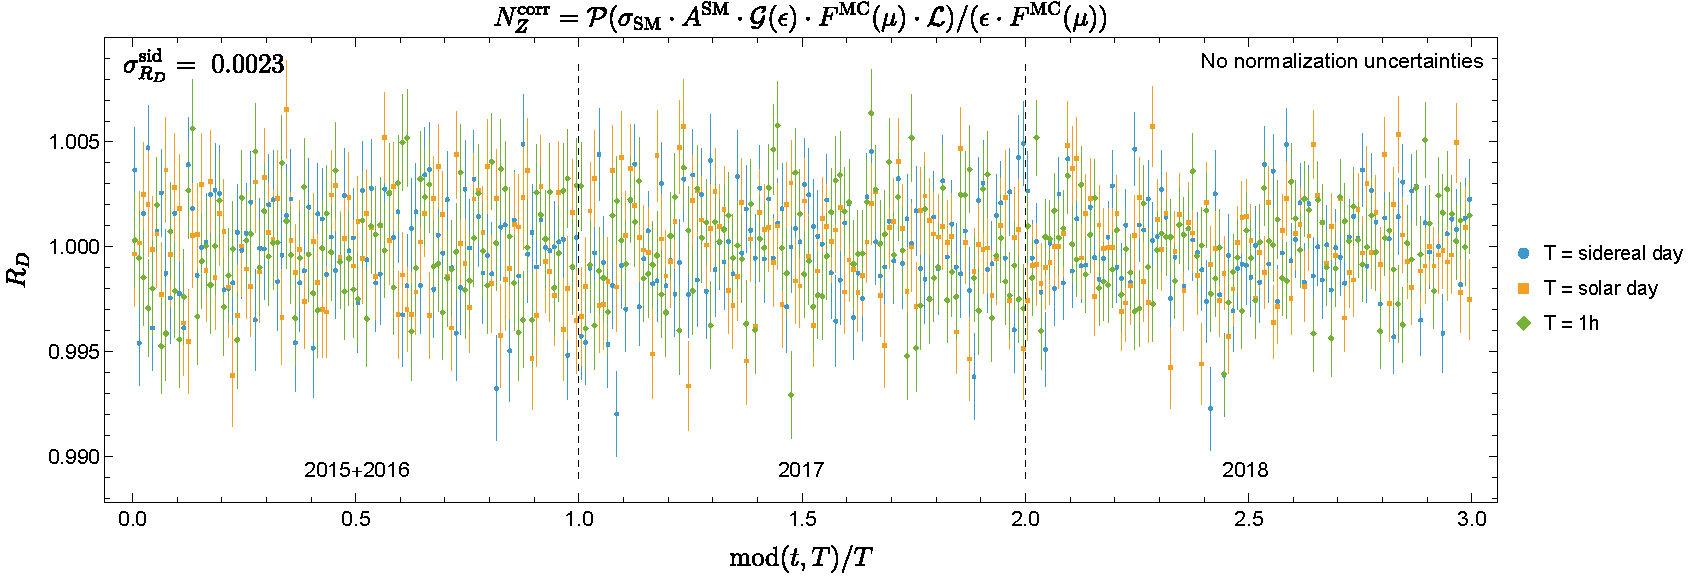
\includegraphics[width=\textwidth]{figs/Mathematica-oldchi2/xs(sigmaFID eps FMC)_noFMCErr_phase}
\caption{$R_D$ distribution for the toy study described in the text. In the upper right corner we show the standard deviation of the sidereal day distribution.}
\label{fig:RD_noFMCerrors}
\end{figure}

\begin{figure}[H]
\centering
\begin{minipage}[H]{0.49\textwidth}
    \vspace{1.6cm}
    \centering
    \begin{tabular}{|l|c|}
        \hline
        $d_u^{XZ}$ & $(0.5 \pm 4.0)\times 10^{-6}$ \\
        $d_u^{YZ}$ & $(-5.7 \pm 3.8)\times 10^{-6}$ \\
        $d_u^{XX-YY}$ & $(-2.4 \pm 2.0)\times 10^{-6}$ \\
        $d_u^{XY}$ & $(-1. \pm 9.5)\times 10^{-7}$ \\
        $c_u^{XZ}$ & $(0.4 \pm 3.1)\times 10^{-6}$ \\
        $c_u^{YZ}$ & $(-4.4 \pm 3.0)\times 10^{-6}$ \\
        $c_u^{XX-YY}$ & $(-1.9 \pm 1.5)\times 10^{-6}$ \\
        $c_u^{XY}$ & $(-0.7 \pm 7.4)\times 10^{-7}$ \\
        $c_d^{XZ}$ & $(0.2 \pm 1.4)\times 10^{-4}$ \\
        $c_d^{YZ}$ & $(-2.0 \pm 1.3)\times 10^{-4}$ \\
        $c_d^{XX-YY}$ & $(-8.3 \pm 6.8)\times 10^{-5}$ \\
        $c_d^{XY}$ & $(-0.3 \pm 3.3)\times 10^{-5}$ \\
                \hline
        \end{tabular}
\end{minipage}
\begin{minipage}[H]{0.49\textwidth}
    \vspace{0pt}
    \centering
   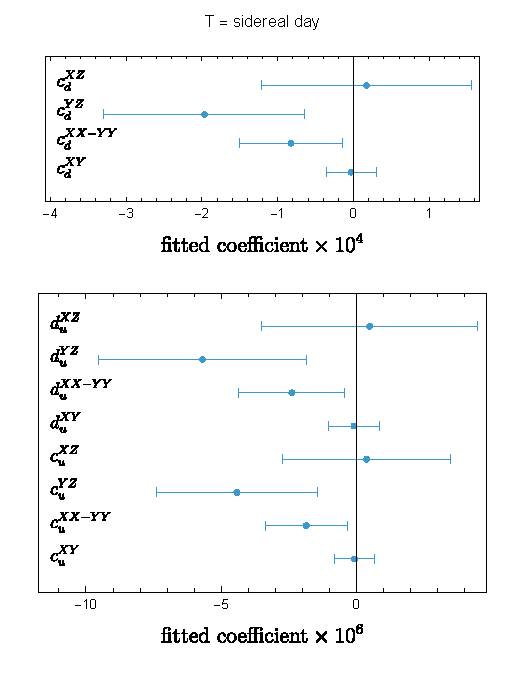
\includegraphics[width=\textwidth]{figs/Mathematica-oldchi2/xs(sigmaFID eps FMC)_noFMCErr_fit}
\end{minipage}
\caption{Fit results for the $N_Z = \sigma_\text{SM}\cdot A^\text{SM} \cdot \epsilon \cdot F^\text{MC}(\mu) \cdot {\cal L}$. No uncertainties on $F^\text{MC}(\mu)$ are included.}
\label{fig:RD_noFMCerrors_fits}
\end{figure}




\subsection{\texorpdfstring{
$N_Z^\text{corr} = \sigma_\text{fid} \cdot \epsilon \cdot F_\text{MC}(\mu)\cdot {\cal L}$ 
with $\delta \epsilon \neq 0$ and $\delta F^\text{MC}(\mu) \neq 0$}{NZcorr = sigmafid * epsilon * FMC * L with delta epsilon != 0 and delta FMC != 0}}
\label{ssec:all_errors_included}
%
We now repeat the study in Sec.~\ref{ssec:no_FMC_errors} but including uncertainties on $F^\text{MC}(\mu)$. This is the most accurate simulation of the expected $Z$ counts that we can produce. There are two effects that play a role: 
%
\begin{enumerate}
    \item The genuine uncertainty on the fitted $F^\text{MC}(\mu)$ function as shown in figure~4 of Ref.~\cite{ATL-DAPR-PUB-2021-001}.
    \item An uncertainty on the normalization which yields $\mu$ and which introduces a $\delta \mu = 1$ (or 1/2) which is 100\% correlated across all LBs in years 2015/2016, 2017 and 2018. 
\end{enumerate} 
%
As of now we do not have a parametrized version of the genuine $F^\text{MC}(\mu)$ uncertainty and we use $\delta \mu = 1$ in each LB as a proxy for the correct uncertainty. As can be seen in figure~4 of Ref.~\cite{ATL-DAPR-PUB-2021-001}, this procedure yields, in first approximation, the correct uncertainty (which, in any case, turns out to be subdominant compared to the uncertainty on the efficiency $\epsilon$). 

The simulated expected number of events and the corrected counts read:
%
\begin{align}
        N_Z (t)  & = {\cal P} \left( \sigma_\text{fid} \cdot {\cal G} (\epsilon,\delta\epsilon) \cdot F^\text{MC}({\cal G}(\mu,\delta \mu)) \cdot {\cal L}\right) , \label{eq:NZfull}\\
        N_Z^\text{corr} (t) & = \frac{N_Z(t)}{(\epsilon \pm \delta \epsilon) \cdot F^\text{MC}(\mu \pm \delta \mu)} .\label{eq:NZcorrfull}
    \end{align}
%
The double ratio $R_D$ is the constructed as in Eq.~(\ref{eq:RD}). The resulting distribution is shown in figure~\ref{fig:RD_Allerrors}. The standard deviation of the 100 bins for this example is $\sigma_{R_D} = 2.4 \times 10^{-3}$. Using the signal formulas discussed in Eqs.~\ref{eq:duXZ}-\ref{eq:cdXY}, we perform a fit to the 12 SME coefficients. The results are shown in figure~\ref{fig:RD_Allerrors_fits}. The central values are not zero because they have been obtained by a single Poisson sampling.

We see that the impact of including the uncertainty on $F^\text{MC}(\mu)$ is negligible. 

\begin{figure}[H]
\centering
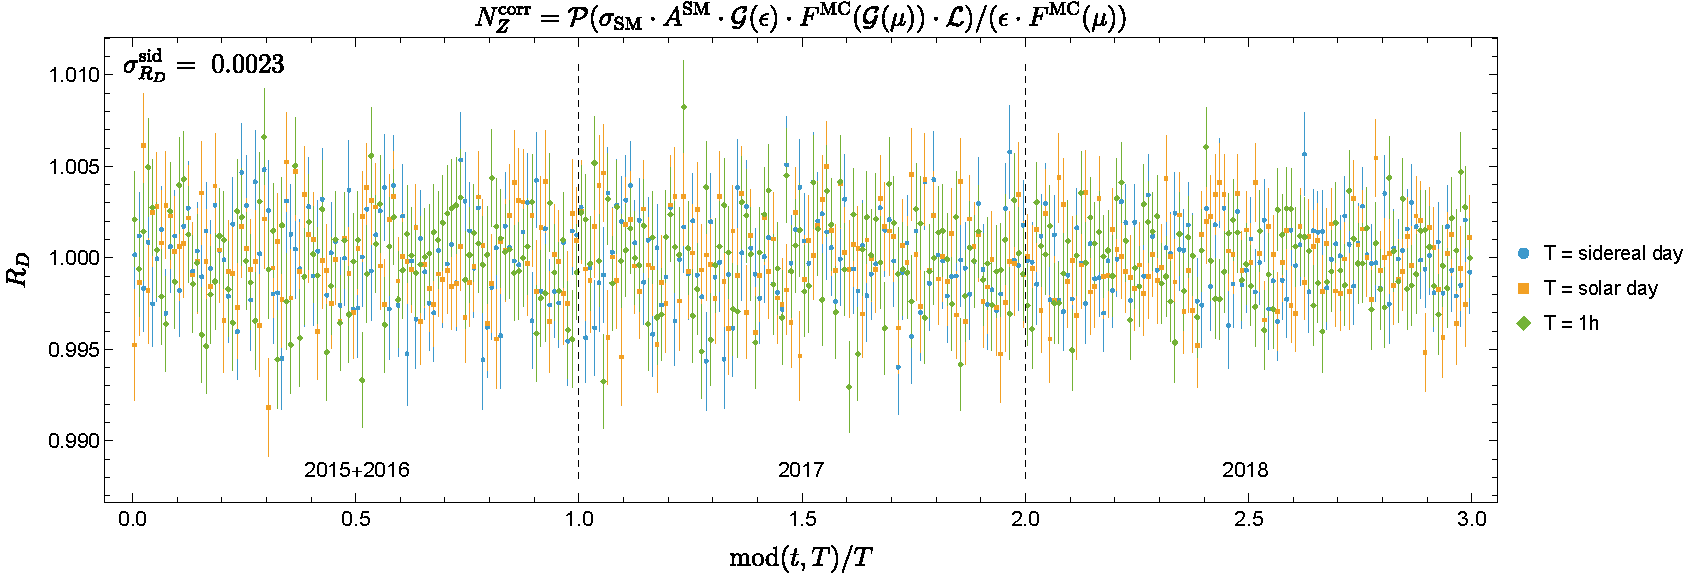
\includegraphics[width=\textwidth]{figs/Mathematica-oldchi2/xs(sigmaFID eps FMC)_phase}
\caption{$R_D$ distribution for the toy study described in the text. In the upper right corner we show the standard deviation of the sidereal day distribution. This is the most accurate simulation of $N_Z$ that we can produce.}
\label{fig:RD_Allerrors}
\end{figure}

\begin{figure}[H]
\centering
\begin{minipage}[H]{0.49\textwidth}
    \vspace{1.6cm}
    \centering
    \begin{tabular}{|l|c|}
        \hline
        $d_u^{XZ}$ & $(-0.7 \pm 4.8)\times 10^{-6}$ \\
        $d_u^{YZ}$ & $(-4.1 \pm 4.6)\times 10^{-6}$ \\
        $d_u^{XX-YY}$ & $(-1.1 \pm 2.4)\times 10^{-6}$ \\
        $d_u^{XY}$ & $(-1. \pm 11.)\times 10^{-7}$ \\
        $c_u^{XZ}$ & $(-0.5 \pm 3.7)\times 10^{-6}$ \\
        $c_u^{YZ}$ & $(-3.2 \pm 3.6)\times 10^{-6}$ \\
        $c_u^{XX-YY}$ & $(-0.8 \pm 1.8)\times 10^{-6}$ \\
        $c_u^{XY}$ & $(-1.0 \pm 8.9)\times 10^{-7}$ \\
        $c_d^{XZ}$ & $(-0.2 \pm 1.7)\times 10^{-4}$ \\
        $c_d^{YZ}$ & $(-1.4 \pm 1.6)\times 10^{-4}$ \\
        $c_d^{XX-YY}$ & $(-3.7 \pm 8.1)\times 10^{-5}$ \\
        $c_d^{XY}$ & $(-0.4 \pm 4.0)\times 10^{-5}$ \\
                                \hline
        \end{tabular}
\end{minipage}
\begin{minipage}[H]{0.49\textwidth}
    \vspace{0pt}
    \centering
   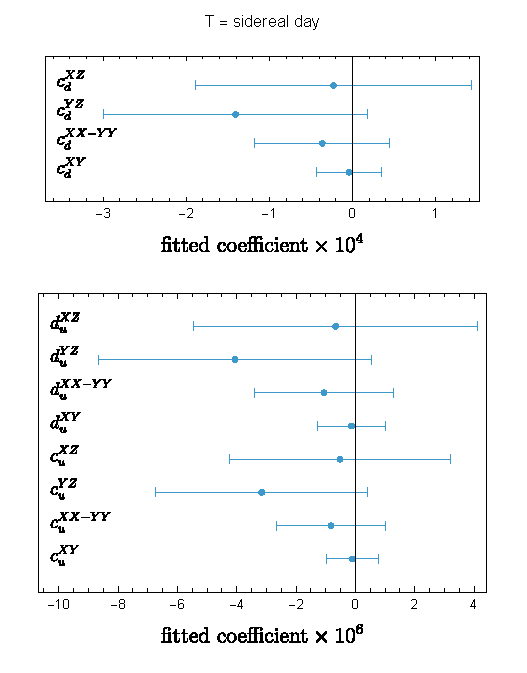
\includegraphics[width=\textwidth]{figs/Mathematica-oldchi2/xs(sigmaFID eps FMC)_fit}
\end{minipage}
\caption{Fit results for the $N_Z = \sigma_\text{SM}\cdot A^\text{SM} \cdot \epsilon \cdot F^\text{MC}(\mu) \cdot {\cal L}$. All sources of uncertainties are included. These results are based on the most accurate simulation of $N_Z$ that we can produce.}
\label{fig:RD_Allerrors_fits}
\end{figure}

\begin{figure}[H]
\centering
\includegraphics[width=\textwidth]{figs/Mathematica-oldchi2/NZ_over_time.pdf}
\caption{Expected number of $Z$ events (before efficiencies corrections) per LB. The LBs are time ordered.}
\label{fig:NZ_over_time}
\end{figure}